\chapter{Analysis of the social network \Twitter}
\label{chapter:analysis}

The work now wants to take a closer look at a concrete social network.
There are of course many social networks, which can be used for harvesting
data, however, as a case study, the author wants to concentrate on a big social
network, which is widely used by employees and individuals. Moreover,
an \textit{API} is needed to gather data automatically.

As a case study, the author had the choice between \textit{Facebook} and
\Twitter. Both are widely used, however \Twitter{} was chosen due to many
already existing programs and platform bindings. Furthermore \Twitter{} is
somewhat more dynamic than \textit{Facebook}, as it offers the possibility to
parse \Twitter{} messages and not just handling static data.

\Twitter{} is a popular social networking and micro-blogging service, that
enables users to post messages and to let other users follow those messages.
The term \textit{micro-blogging} describes a form of communication, that
consists of brief messages in text form, which then can be send over a variety
of ways, like instant messages, mobile phones, e-mail or other \cite{java2007}.

\begin{figure}[hbt]
  \centering
  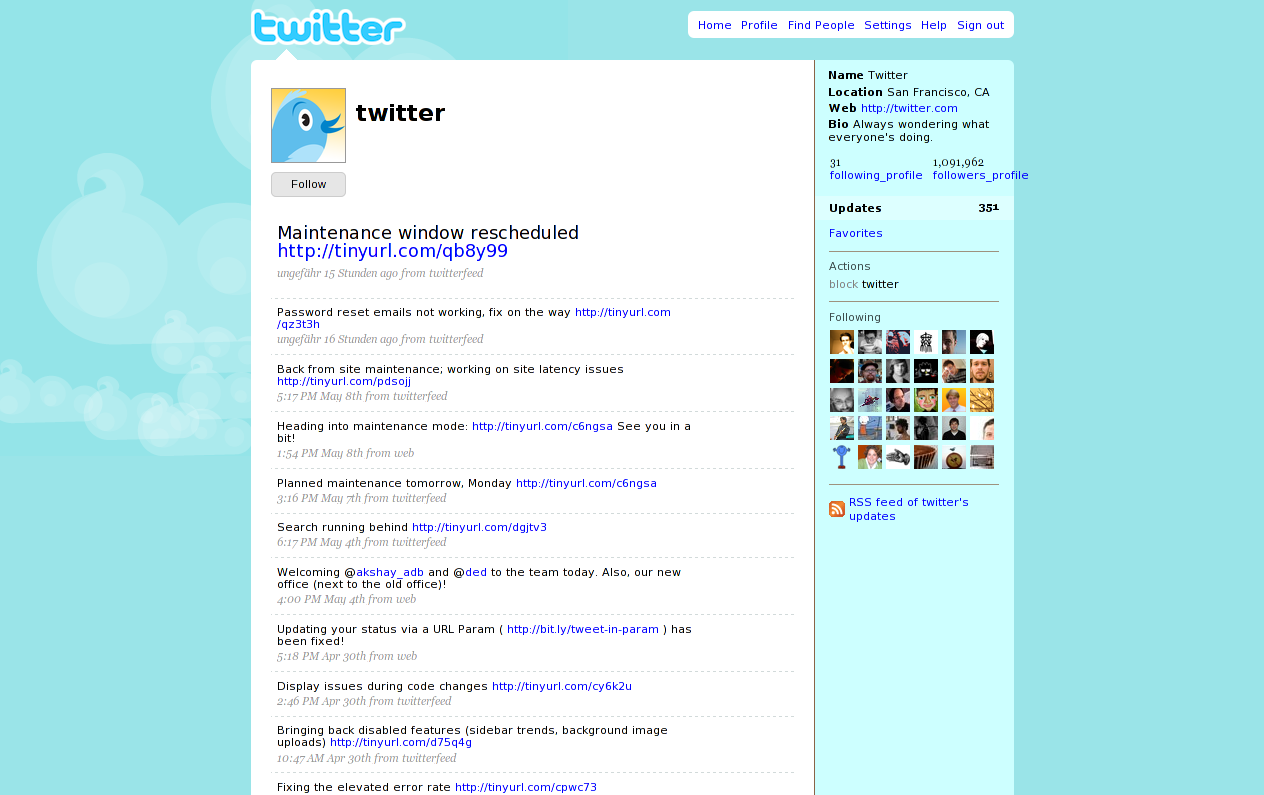
\includegraphics[width=\textwidth]{twitter_screenshot}
  \caption{An example Twitter Homepage, featuring several \Twitter{}
  messages, account information and the users this account
  follows.}\label{fig:twitter_screenshot}
\end{figure}

Micro-blogging itself is relatively new, though already widely used and
provided by services like
\textit{Twitter}\footnote{http://www.twitter.com},
\textit{identi.ca}\footnote{http://identi.ca},
\textit{Jaiku}\footnote{http://www.jaiku.com} and others. \Twitter{} is one of
the most popular micro-blogging services \cite{java2007} and currently
exhibiting more than a million users. The accurate number unfortunately is not
available, however \cite{krishnamurthy2008} estimated about 1.4 million users
in 2008 and \cite{whitworth2009} calculated more than 1.78 million users in
2009.

\Twitter{} limits the length of the messages to 140 characters. The messages
are called \textit{updates} or \textit{tweets}.  The scopes of those messages
range from events, news, daily life and other interests \cite{java2007}. Of
course, other services like Instant Messaging also offers a way to communicate
the such informations, however micro-blogging allows to do this publicly.

As \cite{java2007} describes, micro-blogging is a faster way to communicate
compared to other means of communication, like blogging. It requires less time
to think and write a message, and this of course implements much quicker
\flqq{}write rate\frqq{}. This is of course one of the main differences
between blogging and micro-blogging, whereas an author spends several minutes
to hours to think up and write a blog post. As it now takes less time to think
and write a message, the frequency one can write such, increases and a
micro-blogger may posts several messages a day.

\cite{java2007} has found, that the types of user interactions are daily
chatter, conversations, sharing informations and reporting news. This of course
leads us to question, which information can be dangerous and which can be used
by a social engineer.

\begin{figure}[hbt]
  \centering
  \begin{tikzpicture}[scale=0.75, transform shape,
                      root concept/.append style={concept color=skyblue1},
                      level 1 concept/.append style={concept color=chameleon2},
                      text=white, mindmap]

    \tikzstyle{every annotation}=[fill=skyblue3, font=\sf]

    \node[concept] (Twitter) {Twitter}
      child[concept, grow=160] {node [concept] {Web Interface}}
      child[concept, grow=125] {node [concept] {Twitter API}
      child[concept, grow=left] {node [concept] {User Applications}}}
      child[concept, grow=90] {node [concept] {Facebook}}
      child[concept, grow=55] {node [concept] (top) {IM}}
      child[concept, grow=20] {node [concept] {SMS}}
      %
      child[concept, grow=200] {node [concept] {Web Interface}}
      child[concept, grow=235] {node [concept] {Twitter API}
      child[concept, grow=170] {node [concept] {RSS}}
      child[concept, grow=210] {node [concept] {User Applications}}}
      child[concept, grow=270] {node [concept] {Facebook}}
      child[concept, grow=305] {node [concept] (bottom) {SMS}}
      child[concept, grow=340] {node [concept] {IM}};

    \node[annotation] at (52.5:7.5) {Twitter Input Methods};
    \node[annotation] at (307.5:7.5) {Twitter Output Methods};

    \draw (2,0) -- (6,0);
    \draw (-2,0) -- (-6,0);

  \end{tikzpicture}
  \caption{\Twitter{} input and output methods, on the basis of \cite{krishnamurthy2008}.}
  \label{fig:twitter_io}
\end{figure}

A sample \Twitter{} profile page is shown in Figure
\ref{fig:twitter_screenshot}. It features several elements, which we will
discuss in the next section. 

\Twitter{} messages can be sent and received by a variety of methods, all
listed in Figure \ref{fig:twitter_io}. Several of those are or were
discontinued for a certain amount of time, but either re-enabled or provided by
a third party company.

\section{\Twitter{} profile data}

As already mentioned, a \Twitter{} profile page consists of a series of
elements, which can be used for harvesting data. We now want to take a closer
look at those elements, the content and how a social engineer can extract data
out of those fields.

\begin{description}[\setlabelphantom{More Info URL}]
\item[Name] This fields tells the real name of a user, it is limited to 20
            characters. It is required to enter a name, albeit a bogus name is
            also accepted. The field is required.\\
            \textit{Example: Peter Sample}
\item[Username] The username is presented with this field. A username is needed
                to create an URL, which is of the form \url{http://www.twitter.com/[username]}.
                Therefore only letters, numbers and underscore are allowed. The maximum length
                is set to 15 characters. The field is required.\\
                \textit{Example: petersample}
\item[E-mail] Though not visible publicly, a \Twitter{} user has to provide an
              e-mail address. As described by \cite{brown2008}, though not provided an e-mail
              address can be build out of a naming scheme and the already
              given data, like the username and the real name. If the user
              is an employee of a certain company, this might be even easier,
              as companies often have certain naming schemes. The field is required.\\
              \textit{Example: petersample@example.com}
\item[More Info URL] The URL is used to link a visitor of a profile to further
                     websites, like the blog of the owner. It can link to
                     any site on the internet. The shown component of the
                     URL is 17 characters. Except XSS prevention,
                     \Twitter{} does not rewrite of the URL, and port numbers
                     after the TLD, spaces, German umlauts and UTF-8 characters were
                     accepted.\\
                     \textit{Example:} \url{http://www.petersample.com/},\\
                     \texttt{http://www.peter sample.com:8080/äöü$\Gamma\Lambda\Sigma\Psi$.htm}
\item[One Line Bio] A short sentence can be shown on the profile page, where a
                    user can describe himself. It it limited to 160 characters.
                    \textit{Example: I am a computer science expert and work
                    for example.com}
\item[Location] The location will also be shown on the profile page and is
                limited to 30 characters.
                \textit{Example: Munich}
\item[Picture] A user can insert a picture of himself, although it is not
               required to do so. Moreover, if a user publishes an image, it does not have to
               show himself, but can also be anything else.
\item[Following] Describes a list of users, the profile owner is \textit{following}.
                 To see the list, one has to be logged in.
\item[Followers] This gives us a list of users on the \Twitter{} network, who
                 are \textit{following} the profile owner. To see the list, one has to be logged in.
\item[Favorites] A user can mark his messages as a favorite, which displays a
                 yellow star beneath them. A users favorite messages can be viewed
                 by visiting \url{http://twitter.com/favorites?user=[username]}.
\item[Messages] Finally the messages, which are composed by the actual message,
                which is limited to 140 characters, the time, when the message
                was written and by which mean. A message is identified by a unique
                id, e.g. 1767572233 and can be accessed by
                \url{http://twitter.com/[username]/status/[message id]}.
\end{description}


\section{Threats and risks}

\section{Relevant data and the security risks of those at individuals and companies}
\subsection{The challenge of extracting data automatically}
\subsection{Ontology and classification of the data}
\subsection{Automatic extraction and evaluation}

\section{Accomplishment of attacks}

\section{Countermeasures}
